

\begin{figure*}[t!]
    \centering
    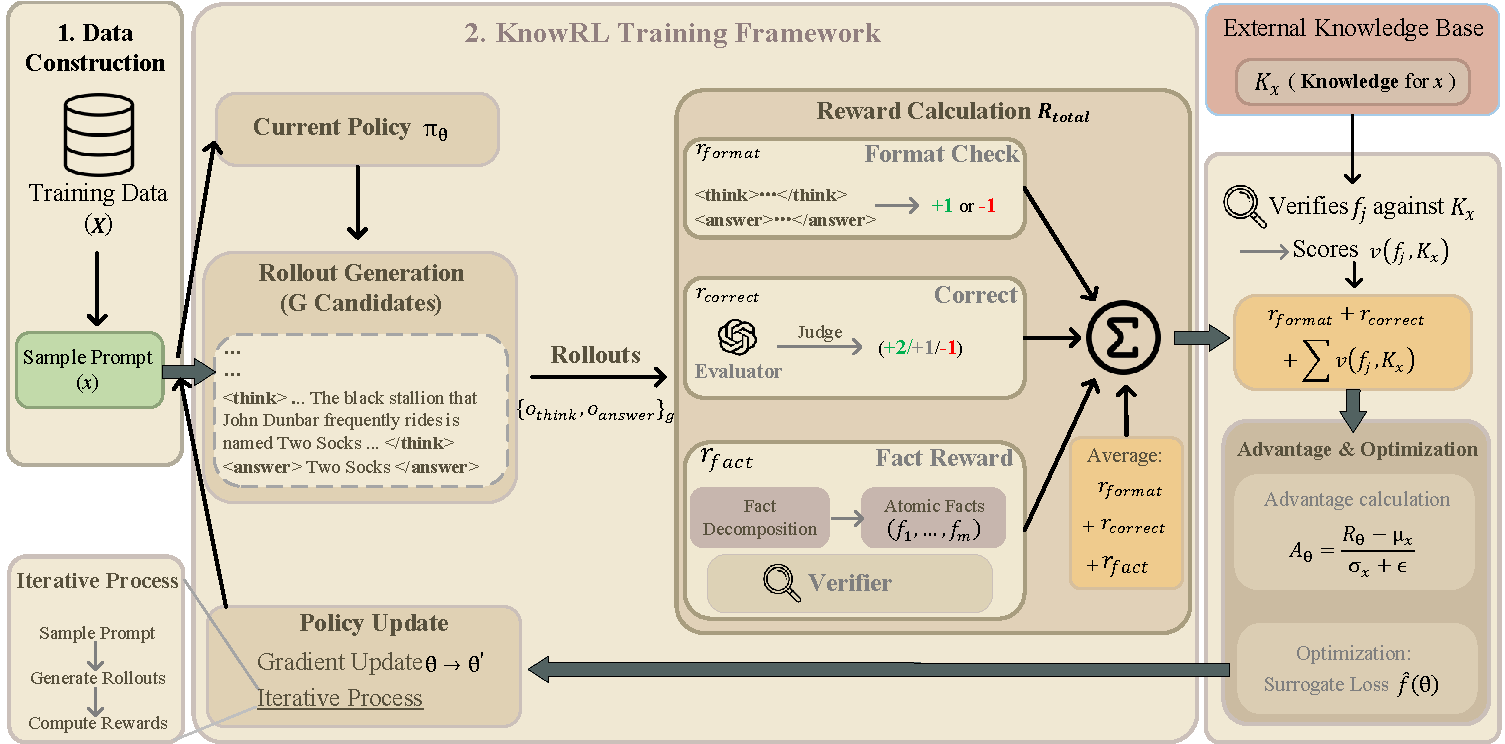
\includegraphics[width=1.0\linewidth]{images/framework1.pdf}
    % \vspace{-2ex}
    \caption{\textbf{Overview of the KnowRL framework.} We first construct training data matched with external knowledge. During RL training, we decompose the generated reasoning process into atomic facts and verify them against the knowledge base. Finally, we optimize the model using a composite reward that combines these factual scores with correctness and format checks.}
    % \vspace{-3ex}
    \label{knowrl}
\end{figure*}

\section{Knowledgeable Reinforcement Learning}

To address the high hallucination rates in slow-thinking models, we propose a fundamental shift in supervision: focusing on the \textbf{\textit{reasoning process}} rather than only on final outcomes. 
To this end, we introduce \texttt{KnowRL}, a Knowledge enhanced Reinforcement Learning framework designed to guide models toward verifiable and boundary-aware reasoning by integrating factual supervision directly into the RL loop. 
As illustrated in Figure~\ref{knowrl}, we first construct training data matched with knowledge, and then conduct RL training using a composite reward that balances factual correctness with reasoning quality (details in Appendix~\ref{appendix:data-construction}). 
By enforcing factual consistency at the step level, KnowRL effectively corrects incorrect reasoning paths and encourages models to recognize their \textbf{\textit{knowledge boundaries}}, ultimately leading to a more faithful and self-aware thinking process.





KnowRL builds upon the Group Relative Policy Optimization (GRPO) algorithm by introducing \emph{factuality supervision} into the CoT reasoning process. This integration ensures that the model is guided not just by the final answer, but by the factual accuracy of its thinking steps. In the following, we detail how we design the composite Reward Function to evaluate these steps and how we implement the Factuality-Guided Policy Optimization.

\medskip
\noindent\textbf{Reward Function.}  
Given a rollout \(o=(o_{\mathrm{think}},o_{\mathrm{answer}})\), inspired by FactScore~\citep{min2023factscore}, we use GPT-4o-mini for the factual verification process. 
We decompose the reasoning trace into \(M\) atomic facts \(\Phi(o_{\mathrm{think}})=\{f_1,\dots,f_M\}\). 
Given an external knowledge base $K$, each atomic fact $f_j$ is checked against its most relevant knowledge set $K_x \subseteq K$\footnote{Retrieved using \texttt{sentence-transformers/gtr-t5-large}.} to obtain a verification score $v(f_j, K_x) \in \{0,1\}$.
The factuality reward is then defined as the proportion of supported facts:
\begin{equation}
\label{eq:factual-score}
r_{\mathrm{fact}}(o)=
\begin{cases}
\displaystyle \frac{1}{M}\sum_{j=1}^{M}v(f_j,K_x), & M>0,\\[6pt]
0, & M=0 .
\end{cases}
\end{equation}

Additional components include a \emph{\textbf{format reward}} \(r_{\mathrm{format}}(o)\) and a \emph{\textbf{correct reward}} \(r_{\mathrm{correct}}(o)\). 
The format reward verifies whether the output follows the required \texttt{<think>...</think><answer>...</answer>} structure: if the format is valid, \(r_{\mathrm{format}}(o)=+1\); otherwise, \(r_{\mathrm{format}}(o)=-1\). 
The correctness reward evaluates the final answer \(o_{\mathrm{answer}}\) using an evaluator model (GPT-4o-mini): if the answer is correct, \(r_{\mathrm{correct}}(o)=+2\); if the model explicitly refuses, \(r_{\mathrm{correct}}(o)=+1\); if the answer is incorrect, \(r_{\mathrm{correct}}(o)=-1\). 
The composite reward is then defined as
\begin{equation}
R_{\mathrm{total}}(o) = r_{\mathrm{format}}(o) + r_{\mathrm{correct}}(o) + r_{\mathrm{fact}}(o).
\end{equation}




\medskip
%\noindent\textbf{Factuality-Aware GRPO Training.}\;

\noindent\textbf{Factuality–Guided Policy Optimisation.}\;
For every prompt $x$ the current policy
$\pi_{\theta_{\text{old}}}$ generates a \emph{group} of $G$ candidate
roll-outs
$\{o^{(g)}\}_{g=1}^{G}\!\sim\!\pi_{\theta_{\text{old}}}(\cdot|x)$, where
$G$ is the group size. 
Each trajectory is scored by the composite reward
$R_{\mathrm{total}}(\cdot)$, yielding a set of scalars
$\mathcal{R}_x=\{R_g\}_{g=1}^{G}$.

\noindent\textbf{Advantage construction.}
We summarise $\mathcal{R}_x$ with its sample mean
$\mu_{x}$ and standard deviation $\sigma_{x}$. 
The credit assigned to trajectory $g$ is the
\emph{group-relative advantage}
\begin{equation}
\label{eq:adv}
A_{g}\;=\;\frac{R_{g}-\mu_{x}}{\sigma_{x}+\varepsilon},
\end{equation}
where $\varepsilon\!(\!\ll\!1)$ avoids division by~zero.
$A_{g}$ is positive if $o^{(g)}$ attains above-average factual reward and negative otherwise, turning factual supervision into a signed learning signal.

\noindent\textbf{Likelihood ratio.}
Define the trajectory-level importance ratio
\[
\varrho_{g}
=\frac{\pi_{\theta}\!\bigl(o^{(g)}\!\mid x\bigr)}
       {\pi_{\theta_{\mathrm{old}}}\!\bigl(o^{(g)}\!\mid x\bigr)}.
\]
The pair $(\varrho_{g},A_{g})$ fully characterises how $o^{(g)}$ should
influence the update: \emph{increase} its probability if
$\varrho_{g}A_{g}>0$ and \emph{decrease} otherwise.

\noindent\textbf{Surrogate objective.}
Using these short symbols enables a compact, column-friendly surrogate:
\begin{equation}
\label{eq:surrogate}
\hat{\mathcal{J}}(\theta)=
\frac{1}{G}\sum_{g=1}^{G}
\min\!\bigl(
      \varrho_{g}A_{g},\,
      \operatorname{clip}(\varrho_{g},1-\epsilon,1+\epsilon)A_{g}
     \bigr),
\end{equation}
with a small clip threshold $\epsilon$ to bound the update.
Because $A_{g}$ encodes factual advantage,
maximising $\hat{\mathcal{J}}$ explicitly transfers probability mass from hallucination-heavy traces ($A_{g}<0$) to trajectories whose CoT is knowledge-supported ($A_{g}>0$).


\noindent\textbf{Regularised loss.}\;
To preserve exploration and limit divergence from the frozen reference policy $\pi_{\text{ref}}$, we add (i) an entropy bonus and (ii) a KL anchor.  
Let $o$ denote a complete rollout and $o_t$ its $t$-th token.  
The token-level Shannon entropy on prompt $x$ is therefore
$\mathcal{H}(\pi_{\theta}(\cdot|x))
      =-\sum_{t}\pi_{\theta}(o_t|x)\log\pi_{\theta}(o_t|x)$.
Its mini-batch expectation and the corresponding KL expectation are
$\mathcal{E}_{\mathcal{H}}\triangleq\mathbb{E}_{x}[\mathcal{H}(\pi_{\theta}(\cdot|x))]$ and
$\mathcal{E}_{\mathrm{KL}}\triangleq\mathbb{E}_{x}[D_{\mathrm{KL}}(\pi_{\theta}(\cdot|x)\|\pi_{\text{ref}}(\cdot|x)]$.
With scalar weights $\beta_{\mathcal{H}},\beta_{\mathrm{KL}}>0$, the final objective becomes
\begin{equation}
\label{eq:loss}
\mathcal{L}_{\text{KnowRL}}
  = -\hat{\mathcal{J}}(\theta)
    \;+\;\beta_{\mathcal{H}}\mathcal{E}_{\mathcal{H}}
    \;+\;\beta_{\mathrm{KL}}\mathcal{E}_{\mathrm{KL}}.
\end{equation}


During training, each gradient step proceeds as follows.  
First, a mini-batch of prompts $x$ is sampled and the old policy
$\pi_{\theta_{\mathrm{old}}}$ produces a group $\mathcal{O}_x$ of
$G$ roll-outs.
Next, every trajectory $o^{(g)}\!\in\!\mathcal{O}_x$ undergoes the
knowledge check that yields the composite reward
$R_g=R_{\mathrm{total}}(o^{(g)})$, whose factual component
$r_{\text{fact}}$ is computed against the external knowledge base.
The set $\{R_g\}$ is then converted into group-relative advantages
$A_g$ via Eq.\,\eqref{eq:adv}, so that a higher proportion of verified
facts directly translates into a larger positive $A_g$, whereas
hallucinated chains of thought receive negative credit.
The new policy $\pi_{\theta}$ is updated by maximising the factual
surrogate $\hat{\mathcal{J}}(\theta)$ in Eq.\,\eqref{eq:surrogate}
while minimising the regularised loss
$\mathcal{L}_{\text{KnowRL}}$ in Eq.\,\eqref{eq:loss};
this couples the likelihood ratio $\varrho_g$ with $A_g$ so that
gradients \emph{increase} the probability of
knowledge supported reasoning and \emph{decrease} that of
hallucination prone trajectories.  
Iterating this loop prompt sampling, factual verification,
advantage normalisation, and loss-driven update---yields a policy that
systematically suppresses hallucinations yet preserves answer accuracy.




% KnowRL is a factuality supervised variant of GRPO. By rewarding the proportion of correct atomic facts in chain-of-thought and integrating entropy-aware regularization, it encourages models to \emph{think factually} while maintaining exploration, effectively mitigating hallucinations in slow-thinking models.










































% \subsection{Reward Function Design}
% We design a special reward function to guide the model in generating outputs that are not only factual in the reasoning process but also provide accurate final answers. 
% The final reward for a model output \(o\) is denoted as \(R_{\text{total}}(o)\).

% \paragraph{Format Reward.}
% The format reward is to justify the specific \texttt{<think>}$o_{\text{think}}$\texttt{</think>} and \texttt{<answer>}$o_{\text{answer}}$\texttt{</answer>} structure, where \(o_{\text{think}}\) denote the thinking process and \(o_{\text{answer}}\) denote the final answer.
% \begin{equation}
% \label{eq:reward_format}
% R_{\text{format}}(o) = \begin{cases} +1 & \text{if } o \text{ has valid format} \\ -1 & \text{otherwise} \end{cases}.
% \end{equation}

% \paragraph{Correct Reward.}
% The correct reward evaluates the accuracy of the final answer \(o_{\text{answer}}\), which is assessed by the GPT-4o-mini. 
% A model's response can be correct, incorrect, or a refusal, and as shown in~\eqref{eq:reward_correct}, both incorrect answers and refusals receive -1 penalty from the correctness reward component.
% \begin{equation}
% \label{eq:reward_correct}
% R_{\text{correct}}(o) = \begin{cases} +2 & \text{if } o_{\text{answer}} \text{ is correct} \\ -1 & \text{otherwise} \end{cases}.
% \end{equation}

% \paragraph{Fact Reward.}
% The fact reward quantifies the factuality of the reasoning process articulated in \(o_{\text{think}}\). 
% We achieve this by using FactScore, which decomposes \(o_{\text{think}}\) into atomic facts and verifies their support against an external knowledge base \(K\). 
% We use the Wikipedia text matched with each entry in the training data to construct \(K\). 
% We first utilize GPT-4o-mini to decompose the input text into several atomic facts. 
% Subsequently, we use an NLI model\footnote{The DeBERTa-v3-base-mnli-fever-anli model.} to determine if each atomic fact is supported by text retrieved from the \(K\). 
% \(N_{\text{supported}}(o_{\text{think}}, K)\) is the number of atomic facts in \(o_{\text{think}}\) supported by \(K\). 
% \begin{equation}
% \label{eq:reward_fact}
% R_{\text{fact}}(o) = \min\left(\frac{N_{\text{supported}}(o_{\text{think}}, K)}{15}, 1.0\right).
% \end{equation}
% This encourages the model to ground its reasoning in verifiable facts.

% The \(R_{\text{combined}}(o)\) is then formulated to avoid excessively penalizing factual reasoning when the final answer is incorrect:
% \begin{equation}
% \label{eq:reward_combined}
% \resizebox{0.9\hsize}{!}{$
% R_{\text{combined}}(o) = \begin{cases} 
%   +2 & \text{if } o_{\text{answer}} \text{ is correct} \\ 
%   -1 + R_{\text{fact}}(o) & \text{if } o_{\text{answer}} \text{ is incorrect} 
% \end{cases}$}.
% \end{equation}
% This ensures that even if an answer is marked incorrect, the model can still receive a relatively positive reward based on the factuality of its thought.
% % Given that all weights (\(w_{\text{format}}, w_{\text{combined}}\)) are set to 1.0
% Finally, the total reward is defined as:
% \begin{equation}
% \label{eq:reward_total}
% R_{\text{total}}(o) = R_{\text{format}}(o) + R_{\text{combined}}(o).
% \end{equation}


% \subsection{RL Training.}
% We first cold-start the model with SFT to establish a more stable foundation for RL training. For the subsequent RL stage, we employ the Group Relative Policy Optimization \citep[GRPO;][]{shao2024deepseekmath} algorithm on our own constructed dataset. The GRPO process optimizes the model's policy using a combination of a correct reward and our designed fact reward. This fact-based reward guidance is crucial, as it teaches the model to ground its reasoning in facts, thereby effectively mitigating hallucination while maintaining or enhancing its reasoning capabilities\footnote{Qwen3 \citep{yang2025qwen3} is also trained through RL with multiple reward combinations. In the same period, we independently propose KnowRL and construct our own training data for factual tasks. We will open source our training data and code.}.

%We briefly introduce it in the following:

% \paragraph{Group Relative Rewards and Advantage ($A_t$).}
% The model first generates multiple candidate inference paths (actions $o_t$) for a given input cue $q_t$ based on the current policy $\pi_\theta$, forming a “response group”.
% We will then evaluate each path using the reward function $R_{\text{total}}(o_t)$. 
% Then, GRPO normalizes these rewards within the group to get a relative advantage $A_t$ for each response. 
% This value-network-free approach quantifies how well a response performed compared to others generated by the same policy for the same input.

% The GRPO method consists of two key components: a clipped policy optimization term that stabilizes training by constraining policy updates, and a gradient regularization term that controls update magnitudes. Together, they optimize the policy model while ensuring reliable reasoning generation—all without requiring a value network.

% \paragraph{Clipped Surrogate Objective.}
% The GRPO objective function aims to improve the policy $\pi_\theta$ by optimizing its parameters $\theta$. 
% The first component for each timestep $t$ is the PPO-style clipped surrogate objective $L^{\text{CLIP}}_t(\theta)$:
% \begin{equation}
% \label{eq:paper_grpo_clip}
% \resizebox{0.95\hsize}{!}{$
% L^{\text{CLIP}}_t(\theta) 
% = \min(r_t(\theta)A_t, \text{clip}(r_t(\theta), 1-\epsilon, 1+\epsilon)A_t).$}
% \end{equation}
% where $r_t(\theta) = \frac{\pi_\theta(a_t|s_t)}{\pi_{\theta_{\text{old}}}(a_t|s_t)}$ is the policy probability ratio, comparing the probability of generating the reasoning path $a_t$ under the current policy $\pi_\theta$ versus the old policy $\pi_{\theta_{\text{old}}}$. 
% $A_t$ is the relative advantage calculated as described above. 
% The $\text{clip}$ function, with a small hyperparameter $\epsilon$, constrains $r_t(\theta)$ to the range $[1-\epsilon, 1+\epsilon]$, ensuring stable updates for learning complex reasoning and factual adherence.

% \paragraph{Gradient Regularization.}
% The second component for each timestep $t$ is the gradient regularization term $L^{\text{REG}}_t(\theta)$ introduced by GRPO:
% \begin{equation} \label{eq:paper_grpo_reg}
% L^{\text{REG}}_t(\theta) = \lambda \|\nabla_\theta r_t(\theta)\|^2.
% \end{equation}
% where $\lambda$ is a regularization coefficient that penalizes large gradients of the policy probability ratio $r_t(\theta)$ with respect to the policy parameters $\theta$. 
% This further constrains the magnitude of policy updates, which is particularly important for GRPO's stability as it operates without a value network.

% The final GRPO objective $L^{\text{GRPO}}(\theta)$ combines these components by taking the expectation over timesteps $t$:
% \begin{equation} \label{eq:paper_grpo_objective}
% L^{\text{GRPO}}(\theta) = \mathbb{E}_t[L^{\text{CLIP}}_t(\theta) - L^{\text{REG}}_t(\theta)].
% \end{equation}
% By optimizing this objective, GRPO guides slow-thinking models to discover and reinforce policies that produce reasoning paths that are not only correct but also fact-based. 


% \begin{table*}[!htbp]
%     \centering
%     \small
%     \setlength{\tabcolsep}{3.2pt}
%     \renewcommand{\arraystretch}{1.2} % Slightly increase row height for readability
%     \begin{tabular}{l|ccc|cc}
%     \toprule
%     \multirow{2}{*}{\makecell[c]{\normalsize\textbf{KnowRL}}} & \multicolumn{3}{c|}{\textbf{Hallucination}} & \multicolumn{2}{c}{\textbf{Reasoning}} \\
%     \cmidrule(lr){2-4} \cmidrule(lr){5-6}
%     & \small\textbf{TruthfulQA} & \small\textbf{SimpleQA} & \small\textbf{ChineseSimpleQA}  & 
%     \small\textbf{GPQA} & \small\textbf{AIME 2025}\\
   
%     \midrule
%     \multicolumn{6}{c}{\textbf{DeepSeek-R1-Distill-Qwen-7B}} \\
%     \text{allbehavior}           & 37.58 & 2.88 & 10.47  & 38.38 & 10.00  \\
%     \text{0.25nobehavior}        & 36.96 & 3.83 & 13.57  & 35.35 & 20.00  \\
%     \text{0.5nobehavior}         & 37.21 & 3.94 & 13.47  & 37.37 & 23.33  \\
%     \text{0.75nobehavior}        & 35.86 & 3.74 & 12.03  & 34.34 & 16.67  \\
%     \text{nobehavior}            & 36.23 & 3.54 & 12.63  & 34.34 & 16.67  \\
%     \bottomrule
%     \end{tabular}
%     \vspace{-1ex}
%     \caption{ Main Experiment}
%     \vspace{-3ex}
%     \label{tab:tofu}
% \end{table*}